\documentclass[tikz,border=6pt]{standalone}
\usepackage{pgfplots}
\pgfplotsset{compat=1.18}
\usepgfplotslibrary{colormaps}
\usetikzlibrary{arrows, arrows.meta, calc}
\usetikzlibrary{decorations.markings}


\usepackage{amssymb,amsmath,mathtools}

\usepackage[T1]{fontenc}
\usepackage[utf8]{inputenc}
\usepackage{newpxtext,newpxmath}
\usepackage{sectsty}

\renewcommand{\Re}{\operatorname{\mathrm{Re}}}
\renewcommand{\Im}{\operatorname{\mathrm{Im}}}

\begin{document}
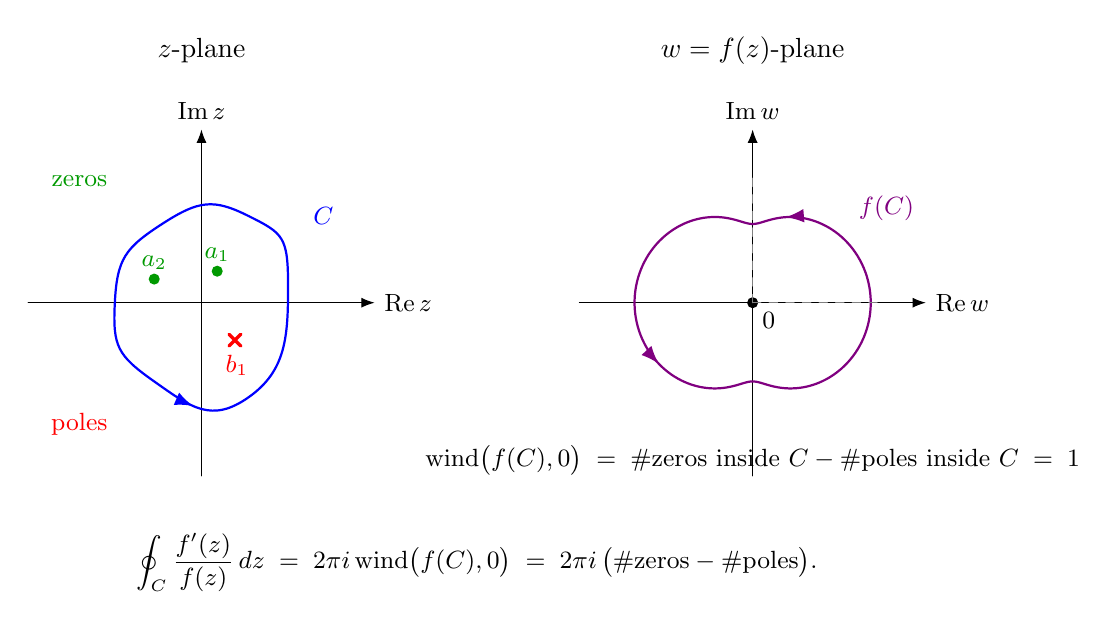
\begin{tikzpicture}[>=Latex, line cap=round, line join=round, font=\small]

%========================
% Left: z-plane
%========================
\begin{scope}[shift={(0,0)}]
	\node[font=\normalsize] at (0,3.2) {$z$-plane};
	% axes
	\draw[->] (-2.2,0)--(2.2,0) node[right] {$\Re z$};
	\draw[->] (0,-2.2)--(0,2.2) node[above] {$\Im z$};
	
	% closed curve C (positively oriented)
	\draw[blue,thick,
	postaction={decorate},
	decoration={markings, mark=at position 0.55 with {\arrow{>}}}]
	plot[smooth cycle, tension=1]
	coordinates{(1.1,0.2) (0.6,1.1) (-0.5,1.0) (-1.1,0.0) (-0.6,-1.0) (0.6,-1.2)};
	\node[blue] at (1.55,1.1) {$C$};
	
	% zeros inside C (green dots)
	\fill[green!60!black] (0.20,0.40) circle(2pt) node[above] {$a_1$};
	\fill[green!60!black] (-0.60,0.30) circle(2pt) node[above] {$a_2$};
	\node[green!60!black] at (-1.55,1.55) {zeros};
	
	% a pole inside C (red cross)
	\draw[red,very thick] (0.35,-0.55) -- (0.50,-0.40);
	\draw[red,very thick] (0.35,-0.40) -- (0.50,-0.55);
	\node[red] at (0.45,-.8) {$b_1$};
	\node[red] at (-1.55,-1.55) {poles};
\end{scope}

%========================
% Right: w-plane = f(z)-plane
%========================
\begin{scope}[shift={(7.0,0)}]
	\node[font=\normalsize] at (0,3.2) {$w=f(z)$-plane};
	% axes
	\draw[->] (-2.2,0)--(2.2,0) node[right] {$\Re w$};
	\draw[->] (0,-2.2)--(0,2.2) node[above] {$\Im w$};
	
	% origin (target of zeros/poles counting)
	\fill (0,0) circle(2pt) node[below right] {$0$};
	
	% image curve f(C) winding once around 0 (violet)
	\draw[violet,thick,
	postaction={decorate},
	decoration={
		markings,
		mark=at position 0.20 with {\arrow{>}},
		mark=at position 0.60 with {\arrow{>}}
	}]
	plot[domain=0:6.283, samples=220]
	({1.25*cos(\x r)+0.25*cos(3*\x r)},
	{1.25*sin(\x r)+0.25*sin(3*\x r)});
	\node[violet] at (1.7,1.2) {$f(C)$};
	
	% helper rays to show angle / winding
	\draw[gray,dashed] (0,0) -- (1.6,0);
	\draw[gray,dashed] (0,0) -- (0,1.6);
	
	% annotation: winding equals zeros minus poles
	\node[align=center] at (0,-2.0)
	{$\mathrm{wind}\big(f(C),0\big)
		\;=\; \#\text{zeros inside $C$} - \#\text{poles inside $C$}
		\;=\; 1$};
\end{scope}

%========================
% Caption (optional)
%========================
\node[align=center] at (3.5,-3.3) {$\displaystyle
	\oint_C \frac{f'(z)}{f(z)}\,dz
	\;=\; 2\pi i\,\mathrm{wind}\big(f(C),0\big)
	\;=\; 2\pi i\,\big(\#\text{zeros}-\#\text{poles}\big).
	$};

\end{tikzpicture}
\end{document}
